\begin{adjustwidth*}{}{-2.25in}
\textbf{{\large Exercises}}
\setlength{\columnsep}{25pt}
\begin{multicols*}{2}
\noindent Terms and Concepts \small

\begin{enumerate}[1)]
\item In your own words, what does it mean to ``find the limit of $f(x)$ as $x$ approaches 3''?
\item An expression of the form $\frac00$ is called \underline{\hskip 15pt}.
\item T/F: The limit of $f(x)$ as $x$ approaches $5$ is always $f(5)$.
\item T/F: If $\ds \lim_{x\to 1^-} f(x) = 5$, then $\ds \lim_{x\to 1} f(x) = 5$.
\item T/F: If $\ds \lim_{x\to 1^-} f(x) = 5$, then $\ds \lim_{x\to 1^+} f(x) = 5$.
\item T/F: If $\ds \lim_{x\to 1} f(x) = 5$, then $\ds \lim_{x\to 1^-} f(x) = 5$.
\item Describe three situations where $\displaystyle \lim_{x\to c}f(x)$ does not exist.
\end{enumerate} 

\noindent {\normalsize Problems\\} \small

\noindent In the following exercises, evaluate each expression using the given graph of $f(x)$.

\begin{enumerate}[1),resume]
\item 
\begin{minipage}{\linewidth}\centering
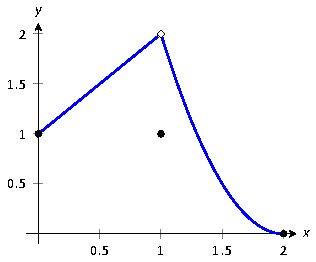
\includegraphics[scale=.8]{figures/fig01_04_ex_05}
\end{minipage}

\noindent\begin{minipage}[t]{.5\linewidth}
\begin{enumerate}
\item		$\ds \lim_{x\to 1^-} f(x)$
\item		$\ds \lim_{x\to 1^+} f(x)$
\item		$\ds \lim_{x\to 1} f(x)$
\end{enumerate}
\end{minipage}
\noindent\begin{minipage}[t]{.5\linewidth}
\begin{enumerate}\addtocounter{enumii}{3}
\item		$f(1)$
\item		$\ds \lim_{x\to 0^-} f(x)$
\item		$\ds \lim_{x\to 0^+} f(x)$
\end{enumerate}
\end{minipage}

\item
\begin{minipage}{\linewidth}\centering
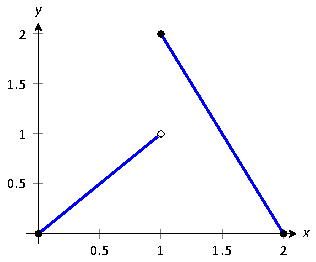
\includegraphics[scale=.8]{figures/fig01_04_ex_06}
\end{minipage}

\noindent\begin{minipage}[t]{.5\linewidth}
\begin{enumerate}
\item		$\ds \lim_{x\to 1^-} f(x)$
\item		$\ds \lim_{x\to 1^+} f(x)$
\item		$\ds \lim_{x\to 1} f(x)$
\end{enumerate}
\end{minipage}
\noindent\begin{minipage}[t]{.5\linewidth}
\begin{enumerate}\addtocounter{enumii}{3}
\item		$f(1)$
\item		$\ds \lim_{x\to 2^-} f(x)$
\item		$\ds \lim_{x\to 2^+} f(x)$
\end{enumerate}
\end{minipage}

\item
\begin{minipage}{\linewidth}\centering
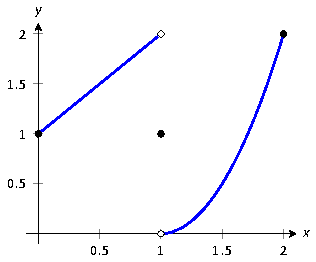
\includegraphics[scale=.8]{figures/fig01_04_ex_08}
\end{minipage}

\noindent\begin{minipage}[t]{.5\linewidth}
\begin{enumerate}
\item		$\ds \lim_{x\to 1^-} f(x)$
\item		$\ds \lim_{x\to 1^+} f(x)$
\end{enumerate}
\end{minipage}
\noindent\begin{minipage}[t]{.5\linewidth}
\begin{enumerate}\addtocounter{enumii}{2}
\item		$\ds \lim_{x\to 1} f(x)$
\item		$f(1)$
%\item		$\ds \lim_{x\to 2^-} f(x)$
%\item		$\ds \lim_{x\to 0^+} f(x)$
\end{enumerate}
\end{minipage}

\end{enumerate}

\vspace{.5cm}

\noindent Using:

\begin{tabular}{lll}
$\ds \lim_{x \to 9}f(x) = 6$ & \quad\quad &$\ds \lim_{x \to 6} f(x) = 9$\\
$\ds \lim_{x \to 9}g(x) = 3$ &  & $\ds \lim_{x \to 6} g(x) = 3$
\end{tabular}

\noindent evaluate the limits given in the following exercises, where possible. If it is not possible to know, state so.
\begin{enumerate}[1),resume]
\item $\ds \lim_{x\to9}(f(x)+g(x))$
\item $\ds \lim_{x\to9}(3f(x)/g(x))$
\item $\ds \lim_{x\to9}\left(\frac{f(x)-2g(x)}{g(x)}\right)$
\item $\ds \lim_{x\to6}\left(\frac{f(x)}{3-g(x)}\right)$
\item $\ds \lim_{x\to9}g\big(f(x)\big)$
\item $\ds \lim_{x\to6}f\big(g(x)\big)$
\item $\ds \lim_{x\to6}g\big(f(f(x))\big)$
\item $\ds \lim_{x\to6}f(x)g(x)-f\,^2(x)+g^2(x)$
\end{enumerate}

\vspace{.5cm}

\noindent Using:

\begin{tabular}{lll}
$\ds \lim_{x\to1}f(x) = 2$ & \quad\quad &$\ds \lim_{x\to10} f(x) = 1$\\
$\ds \lim_{x\to1}g(x) = 0$ &  & $\ds \lim_{x\to10} g(x) = \pi$
\end{tabular}

\noindent evaluate the limits given in the following exercises, where possible. If it is not possible to know, state so.
\begin{multicols}{2}
\begin{enumerate}[1),resume]
\item $\ds \lim_{x\to1}f(x)^{g(x)}$
\item $\ds \lim_{x\to10}\cos \big(g(x)\big)$
\item $\ds \lim_{x\to1}f(x)g(x)$
\item {$\ds \lim_{x\to1}g\big(5f(x)\big)$}
\end{enumerate}
\end{multicols}

\vspace{.5cm}

\noindent In the following exercises, evaluate the limit.
\begin{multicols}{2}
\begin{enumerate}[1),start=23]
\item {$\ds \lim_{x\to3}x^2-3x+7$}
\item {$\ds \lim_{x\to\pi}\frac{3x+1}{1-x}$}
\item {$\ds \lim_{x\to\pi}\frac{x^2+3x+5}{5x^2-2x-3}$}
\item {$\ds \lim_{x\to\pi}\left(\frac{x-3}{x-5}\right)^7$}
\item {$\ds \lim_{x\to\pi/4}\cos x\sin x$}
\item {$\ds \lim_{x\to0}\ln x$}
\end{enumerate}
\end{multicols}

%------------------------------------------
% END OF EXERCISES ON FIRST PAGE
%------------------------------------------
\end{multicols*}
\end{adjustwidth*}

\clearpage

\begin{adjustwidth*}{}{-2.25in}
\setlength{\columnsep}{25pt}
\begin{multicols*}{2}\small

\begin{multicols}{2}
\begin{enumerate}[1),start=29]
\item {$\ds \lim_{x\to3}4^{x^3-8x}$}
\item {$\ds \lim_{x\to\pi/6} \csc x$}
\item {$\ds \lim_{x\to0} \ln(1+x)$}
\item {$\ds \lim_{x\to6^-} \frac{x^2-4 x-12}{x^2-13 x+42}$}
\item {$\ds \lim_{x\to0^+} \frac{x^2+2 x}{x^2-2 x}$}
\item {$\ds \lim_{x\to2^-} \frac{x^2+6 x-16}{x^2-3 x+2}$}
\item {$\ds \lim_{x\to2^+}\frac{x^2-10 x+16}{x^2-x-2}$}
\item {$\ds \lim_{x\to-2}\frac{x^2-5 x-14}{x^2+10 x+16}$}
\item {$\ds \lim_{x\to-1}\frac{x^2+9 x+8}{x^2-6 x-7}$}
\item $\ds \lim_{x \to 1} \frac{x-1}{\sqrt{x} - 1}$
\item $\ds \lim_{x \to 0} \frac{\sqrt{x+4} - 2}{x}$
\item $\ds \lim_{x \to 0} \frac{\sqrt{16 + x} - 4}{x}$
\end{enumerate}
\end{multicols}

\vspace{.5cm}

\noindent Use the Squeeze Theorem, where appropriate, to evaluate the following limits.
\begin{enumerate}[1),start=41]
\item {$\ds \lim_{x \to 0} x \sin\left( \frac{1}{x} \right)$}
\item {$\ds \lim_{x\to0} \sin x\cos\left(\frac{1}{x^2}\right)$}
\item {$\ds \lim_{x\to3} f(x)$, where $x^2\leq f(x) \leq 3x$ on $[0,3]$.}
\end{enumerate}

\vspace{.5cm}

\noindent Using the techniques you learned in Activity~\ref{A:1.1.3} and Activity~\ref{A:1.1.4}, determine the instantaneous velocity of some object with given position function and specific instant.
\begin{enumerate}[1),start=44]
\item $\ds s(t) = -7t + 2; \quad t=3$
\item $\ds s(t) = 9t + 0.06; \quad t=1$
\item $\ds s(t) = t^2 + 3t - 7; \quad t=1$
\item $\ds s(t) = \frac{1}{t+1}; \quad t=2$
\end{enumerate}

%---------------------------------------------
% END OF EXERCISES ON SECOND PAGE
%---------------------------------------------
\end{multicols*}
\end{adjustwidth*}
\afterexercises